\documentclass[
ngerman,
twoside,
pdfa=false,
ruledheaders=section,%Ebene bis zu der die Überschriften mit Linien abgetrennt werden, vgl. DEMO-TUDaPub
class=report,% Basisdokumentenklasse. Wählt die Korrespondierende KOMA-Script Klasse
thesis={type=sta},% Dokumententyp Thesis, für Dissertationen siehe die Demo-Datei DEMO-TUDaPhd
accentcolor=TUDa-2c,% Auswahl der Akzentfarbe
custommargins=false,% Ränder werden mithilfe von typearea automatisch berechnet
marginpar=false,% Kopfzeile und Fußzeile erstrecken sich nicht über die Randnotizspalte
%BCOR=5mm,%Bindekorrektur, falls notwendig
parskip=half-,%Absatzkennzeichnung durch Abstand vgl. KOMA-Sript
fontsize=11pt,%Basisschriftgröße laut Corporate Design ist mit 9pt häufig zu klein
%	logofile=tuda_logo.pdf, %Falls die Logo Dateien nicht installiert sind
]{tudapub}

%%%%%%%%%%%%%%%%%%%%%%%%%%%%
% Download des TU-Logos
%%%%%%%%%%%%%%%%%%%%%%%%%%%%
% https://download.hrz.tu-darmstadt.de/protected/CE/TUDa_LaTeX/tuda_logo.pdf
% Der Pfad zum Logo kann als "logofile" angegeben werden.

%%%%%%%%%%%%%%%%%%%
% Sprachanpassung & Verbesserte Trennregeln
%%%%%%%%%%%%%%%%%%%
\usepackage[english, main=ngerman]{babel}
\usepackage[autostyle]{csquotes}% Anführungszeichen vereinfacht
\usepackage{microtype}

%%%%%%%%%%%%%%%%%%%
% Literaturverzeichnis
%%%%%%%%%%%%%%%%%%%
\usepackage{biblatex}   % Literaturverzeichnis
\addbibresource{HausarbeitBib.bib}

%%%%%%%%%%%%%%%%%%%
% Paketvorschläge Tabellen
%%%%%%%%%%%%%%%%%%%
%\usepackage{array}     % Basispaket für Tabellenkonfiguration, wird von den folgenden automatisch geladen
\usepackage{tabularx}   % Tabellen, die sich automatisch der Breite anpassen
%\usepackage{longtable} % Mehrseitige Tabellen
%\usepackage{xltabular} % Mehrseitige Tabellen mit anpassarer Breite
\usepackage{booktabs}   % Verbesserte Möglichkeiten für Tabellenlayout über horizontale Linien

%%%%%%%%%%%%%%%%%%%
% Paketvorschläge Mathematik
%%%%%%%%%%%%%%%%%%%
\usepackage{mathtools} % erweiterte Fassung von amsmath
\usepackage{amssymb}   % erweiterter Zeichensatz
\usepackage[decimalsymbol=comma]{siunitx}   % Einheiten


%%%%%%%%%%%%%%%%%
% Eigenen Pakete Gruppe03
%%%%%%%%%%%%%%%%%%%%
%\usepackage[utf8]{inputenc}
%\usepackage[ngerman]{babel}
\usepackage{hyperref}
\usepackage{graphicx}
\usepackage{subcaption}
\usepackage{listings}
\usepackage[framed, numbered]{matlab-prettifier}
%\usepackage[style=numeric]{biblatex}
%\usepackage{amsthm}
%\usepackage[squaren]{SIunits}
\usepackage{enumitem}
\usepackage{tikz}
\usepackage{pgfplots}
\usepackage{pgfplotstable}
%\usepackage{booktabs}
\pgfplotsset{compat=1.12}
\usepackage{dsfont}

%%%%%%%%%%%%%%%%%%%
% Pseudocode
%%%%%%%%%%%%%%%%%%%
\usepackage[linesnumbered,lined,boxruled]{algorithm2e} % Package für Pseudocode

%%%%%%%%%%%%%%%%%%%
% Plotting und Grafik
%%%%%%%%%%%%%%%%%%%
\usepackage{tuda-pgfplots} % Package für Plotting with TUDa mods

%%%%%%%%%%%%%%%%%%%
% Sonstiges
%%%%%%%%%%%%%%%%%%%
\usepackage{blindtext} % Package für Blindtext

\begin{document}
	\title{Ausarbeitung Übung 2}
	%\subtitle{Ein Untertitel, wenn nötig}
	\author[D. Schiller, C. Kramer, S.Arnold, T. Lingenberg]{Dominik Schiller \and Constanze Kramer \and Simon Arnold \and Tobias Lingenberg} %optionales Argument ist die Signatur,
	%\reviewer{Gutachter 1 \and Gutachterin 2} %Gutachten
	
	%Diese Felder werden untereinander auf der Titelseite platziert.
	\department{} % Das Kürzel wird automatisch ersetzt und als Studienfach gewählt, siehe Liste der Kürzel im Dokument.

	
	\date{\today}
	%\examdate{\today}
	
	%	\tuprints{urn=1234,printid=12345}
	%	\dedication{Für alle, die \TeX{} nutzen.}
	
	\maketitle
	\pagenumbering{gobble} % Seitenzahlen angezeigt, startet ab dem Inhaltsverzeichnis
	
	
	\affidavit
	%\AffidavitSignature
	%\AffidavitSignature
	
	
	%%%%%%%%%%%%%%%%%%%
	%Abstract / Kurzzusammenfassung
	%%%%%%%%%%%%%%%%%%%
	%\include{chapters/zusammenfassung}
	
	%%%%%%%%%%%%%%%%%%%
	%Inhaltsverzeichnis 
	%%%%%%%%%%%%%%%%%%%
	\cleardoublepage
	\tableofcontents % Erstellte ein Inhaltsverzeichnis
	
	%\cleardoublepage
	\pagenumbering{arabic} % Seitenzahlen angezeigt, startet ab dem Inhaltsverzeichnis
	\setcounter{page}{1} % Setzt den Seitenzahlenzähler auf 1
	
	%%%%%%%%%%%%%%%%%%%%%%%%%%%%%%%%%%%%%%%%%%%%%%%%%%%%%%%%%%%%%%%%%%%%%%%%%%%%%%%%%%%%%%%%%%%%%%%%%%
	
	% INHALT, am Besten ausgelagert in eigene Files/Kapitel und dann mit \include{Unterordner/Filename} eingefügt, sorgt für bessere Übersichtlichkeit und Fehlersuche. Einzelne Dateien sind aktuell im Ordner Sections abgelegt. 
	
	
	%%%%%%%%%%%%%%%%%%Haupteil%%%%%%%%%%%%%%%%%%%
\chapter{Bearbeitung der Aufgaben}
	
	\section*{Harmonischer Oszillator, analytisch, Aufgabe 2.1}\label{sec:ag2.1}
	\begin{figure}[h]
		\centering
		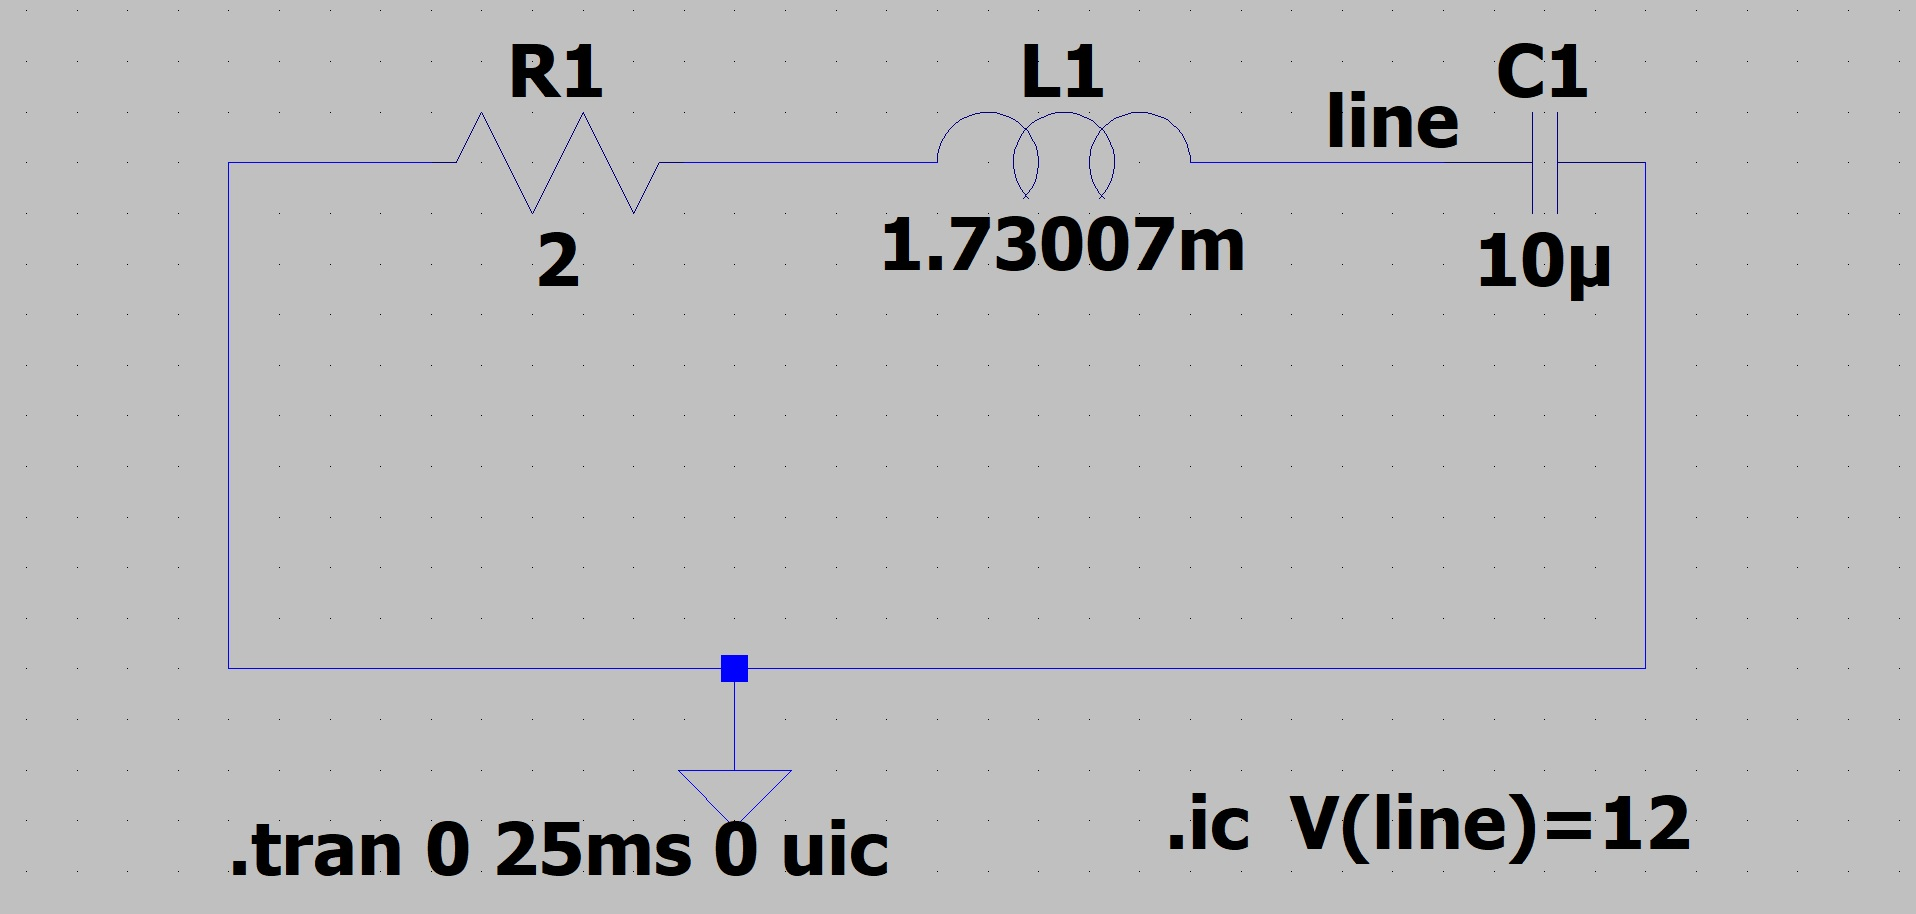
\includegraphics[width=\textwidth]{data/harmOsz}
		\caption{Gegebener harmonischer Oszillator in LT-Spice implementiert}
		\label{oszillator}
	\end{figure}
	Für die vorliegende Schaltung wird angenommen, dass am Kondensator zum Zeitpunkt $t = 0$ eine Spannung $u_\mathrm{C}(0) = 12\,$V anliegt und der Strom durch den Reihenschwingkreis $i(0) = 0\,$A beträgt. Nach dem \textsc{Kirchhoff}'schen Gesetz ergibt sich die Maschengleichung für den Schwingkreis zu $u_\mathrm{C}(t) + u_\mathrm{R}(t) + u_\mathrm{L}(t) = 0$. Aus den Spannungen für den Widerstand $u_\mathrm{R}(t) = R \: i_\mathrm{R}(t)$, die Spule $u_\mathrm{L}(t) = L\: \frac{\mathrm{d}i_\mathrm{L}}{\mathrm{d}t}(t)$ und den Kondensator $u_\mathrm{C}(t) = \frac{1}{C} \int i_\mathrm{C}(t)dt $ ergibt sich daraus die Maschengleichung in Abhängigkeit des Stromes zu 
	
	\begin{equation*}
		R\:i(t) + L\: \frac{\mathrm{d}i}{\mathrm{d}t}(t) + \frac{1}{C} \int i_\mathrm{C}(t)dt = 0.
	\end{equation*}
	
	Nach einmaligem Differenzieren nach der Zeit $t$ folgt daraus die Differentialgleichung 2. Ordnung 
	
	\begin{equation}
		R  \frac{\mathrm{d}i}{\mathrm{d}t}(t) + \frac{1}{\mathrm{C}} i(t) +  L\: \frac{\mathrm{d^2}i}{\mathrm{d}t^2}(t) = 0.
		\label{eq:it1}
	\end{equation}
	
	
	
	Die Lösung der Differentialgleichung im Falle einer gedämpften Schwingung lässt sich aus dem allgemeinen Ansatz 
	
	\begin{equation}
			i(t) = a\mathrm{e}^{(-\delta +j\omega_e)t} + b\mathrm{e}^{(-\delta - j\omega_e)t}
			\label{eq:it2}
	\end{equation}
	
	ermitteln. Hierbei bezeichnet $\delta = \frac{R}{2L}$ die Dämpfung, $\omega_0 = \sqrt{\frac{1}{LC}}$ die Resonanzkreisfrequenz und $\omega_e = \sqrt{\omega_0^2 - \delta^2}$ die gedämpfte Resonanzkreisfrequenz. Die Konstanten $a$ und $b$ werden bestimmt durch einsetzen des Anfangswertes  $i(0) = 0\,$A folgt $a + b = 0$ und somit $a = -b$.\newline
	Da zum Zeitpunkt $t = 0$ noch kein Strom fließt liegt noch keine Spannung $u_\mathrm{R}$ an dem Ohmschen Widerstand $R$ an und somit vereinfacht sich \ref{eq:it1} zu $u_\mathrm{C}(0) +  L\: \frac{\mathrm{d}i}{\mathrm{d}t}(0) = 0$ und durch einsetzen von $u_\mathrm{C}(0) = 12\,$V folgt daraus $L\frac{\mathrm{d}i}{\mathrm{d}t}(0) = -12\:$V. Einmaliges differenzieren von \ref{eq:it2} sowie einsetzen von $ i(0) = 0$ und $a = -b$ ergibt $\frac{\mathrm{d}i}{\mathrm{d}t}(0) = -j2\omega_e b$. Gleichsetzen und nach $b$ auflösen und man erhält $b = -j \frac{u_\mathrm{C}(0)}{2L\omega_e}$ und somit $a = j\frac{u_\mathrm{C}(0)}{2L\omega_e}$. Der Strom ergibt sich damit nun zu 
	
	\begin{equation}
		i(t) = j\frac{u_\mathrm{C}(0)}{2L\omega_e}\mathrm{e}^{(-\delta +j\omega_e)t} - j \frac{u_\mathrm{C}(0)}{2L\omega_e}\mathrm{e}^{(-\delta - j\omega_e)t}.
		\label{eq:it3}
	\end{equation}
	
	Durch einfaches ausmultiplizieren und nutzen der \textsc{Euler}'schen Formel 
	
	\begin{equation*}
		\mathrm{sin}(x) = \frac{\mathrm{e}^{ix} - \mathrm{e}^{-ix}}{2i}
	\end{equation*}
	
	vereinfacht sich \ref{eq:it3} noch weiter zu
	
	\begin{equation*}
		i(t) = -\frac{u_\mathrm{C}}{L\omega_e}\mathrm{e}^{-\delta t}\mathrm{sin}(\omega_et)
	\end{equation*}
	
	Mit den eingebauten Bauelementen $L = 1.73007\:$mH, $R = 2\:\Omega$ und $C = 10 \: \mu $F kommt man auf eine gedämpfte Resonanzkreisfrequenz von $\omega_e = 7580.701\:\mathrm{s}^{-1}$ und eine Dämpfung von $\delta = 578.011\:\mathrm{s}^{-1}$.\newline
	
	Um eine eindeutige Lösung für eine lineare gewöhnliche Differentialgleichung $n$-ter Ordnung zu ermitteln sind auch $n$ Anfangsbedingungen nötig da auch $n$ Integrationen nötig sind um die Differentialgleichung zu lösen und somit auch $n$ Integrationskonstanten bestimmt werden müssen.



	\section{Aufgabe 2.2}\label{sec:ag2.2}
Der in Aufgabe 2.1 vorgestellte harmonische Oszillator soll nun mit Hilfe des Programms \glqq LT-Spice\grqq{} zur Simulation elektrischer Schaltungen nachgebaut und berechnet werden. Da es keine Strom- bzw. Spannungsquelle in der Schaltung gibt, wird am Kondensator eine initiale Spannung zum Zeitpunkt $t = 0$ von 12\volt angelegt. Es handelt sich um eine transiente Simulation, also eine Simulation, bei der zeitabhängige Einflüsse berücksichtigt werden. Der Simulationsbereich bewegt sich zwischen $0$ und $25$ \si{\milli\second}. \\
Die in LT-Spice erzeugte Schaltung wird nun mit der analytisch berechneten Funktion aus Aufgabenteil 1 verglichen. Hierzu sind an verschieden Zeitpunkten $t$ , $t \in [0,25]$ \si{\milli\second} Stromwerte aus dem Graphen in LT-Spice abgelesen worden, sowie die Werte mit Hilfe der Funktion zu gleichen Zeitpunkt $t$ händisch berechnet worden.\\ \\
Daraus ergibt sich die folgende Tabelle\\ \\
\begin{table}[h]
	\centering
	\begin{tabular}[h]{c|c|c}
		Zeitpunkt $t$ in \si{\milli\second} & LT-Spice Wert in \si{\milli\ampere} \ & Berechneter Wert in \si{\milli\ampere} \\
		\hline
		1 & -487,18 & -494,26 \\
		2 & -159,73 & -149,67\\
		3 & 102,45 & 110,23\\
		6 & -28,39 & -28,46\\
		9 & 4,57 & 3,91\\
		12 & -0,356 & -0,122\\
		15 & -0,048 & -0,090\\
	\end{tabular}
\end{table}\\
\\

Zusätzlich zu den Messwerten wurde der Graph der Funktion aus Aufgabenteil 2.1 in Matlab geplottet. Vergleich man nun sowohl die Funktionswerte in der Tabelle, als auch die beiden entstandenen Graphen \ref{lt} und \ref{mat} , so wird deutlich, dass die Funktion aus 2.1 den gleichen Graphen erzeugt wie die Simulation in LT-Spice. Außerdem ist zu erkennen, dass die Amplitude bei fortlaufender Zeit kleiner wird und der Strom gegen $0\:$\si{\milli\ampere} konvergiert. Die Unterschiede in den Funktionswerten der Tabelle lassen sich auf Rundungsfehler, sowie Ablesefehler in LT-Spice zurückführen.
\begin{figure}[h]
	\centering
	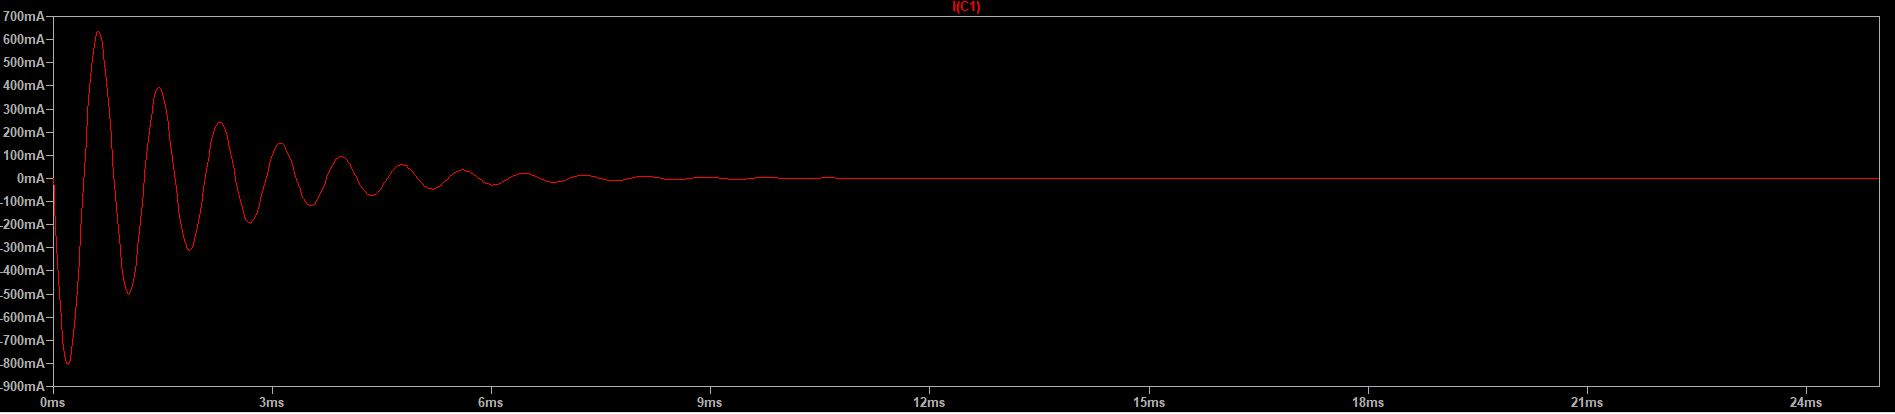
\includegraphics[width=\textwidth]{data/ltsim}
	\caption{Simulationsgraph aus LT-Spice}
	\label{lt}
\end{figure}

\begin{figure}[h!]
	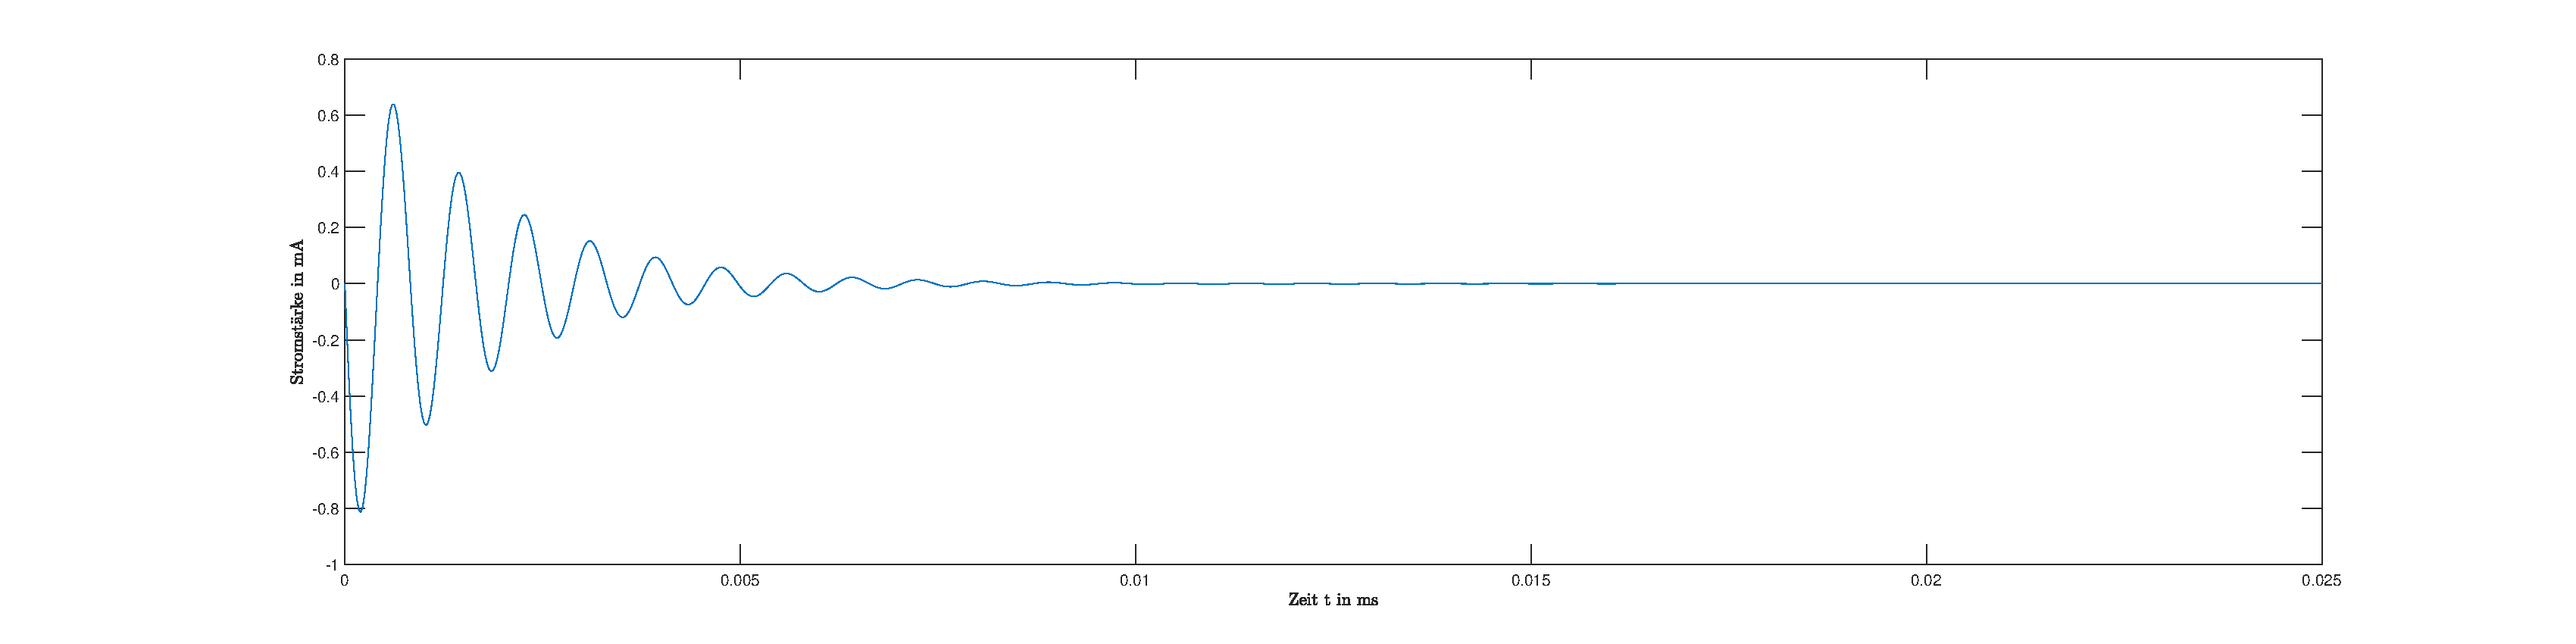
\includegraphics[width=\textwidth]{data/fctmat}
	\caption{Simulationsgraph aus Matlab}
	\label{mat}
\end{figure}
\newpage
Des Weiteren soll untersucht werden, inwiefern sich ein kleinerer Widerstand $R$ auf den Funktionsgraphen auswirkt. Hierzu wurde der Widerstand $R$ in dem harmonischen Oszillator auf den Wert $0,5\:$\si{\ohm} gesetzt. Aus der Graphik \ref{14R} geht hervor, dass die Amplituden durch einen kleineres $R$ beeinträchtigt wird. Wegen der verkleinerten Widerstand nimmt die Auslenkung langsamer ab, gleichzeitig ist der maximal fließende Strom,  höher als der Maximalstrom bei einem größeren Widerstand. Die Periodendauer bleibt unbeeinträchtigt.
\\ \\
\begin{figure}[h]
	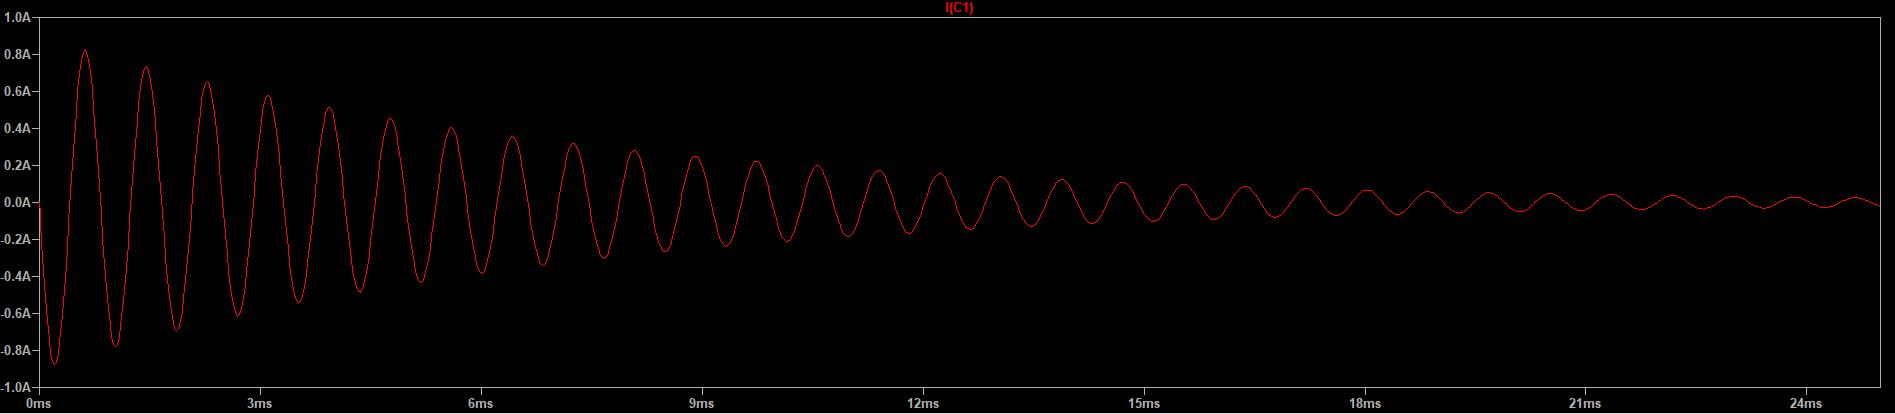
\includegraphics[width=\textwidth]{data/kleineresR}
	\caption{harmonischer Oszillator mit $R = 0,5\:$\ohm}
	\label{14R}
\end{figure}

Neben dem harmonischen Oszillator wird eine weitere Schaltung in LT-Spice betrachtet. Bei dieser Schaltung handelt es sich um einen Spannungsverdoppler. Diese ist auch unter dem Namen Villard-Schaltung bekannt.\\

Wie der Name besagt, ist das Ziel der Schaltung die Ausgangsspannung, im Vergleich zur Eingangsspannung, zu verdoppeln. Bei der gegebenen Schaltung \ref{bspS} handelt es sich nicht um einen Standard Spannungsverdoppler, der nur aus einer Diode und einem Kondensator besteht, sondern um einen von Greinacher erweiterten Spannungsverdoppler . Bei diesem ist der Villard-Schaltung, die aus dem Kondensator C1 und der Diode D1 besteht, noch ein Kondensator C2 und eine Diode D2 nachgeschaltet. Zusätzlich wurde der Widerstand R1 in Reihe zur Spannungsquelle geschaltet. Voraussetzung für Villard-Schaltung ist eine Quelle, die eine Wechselspannung erzeugt. \\

\begin{figure}[h!]
	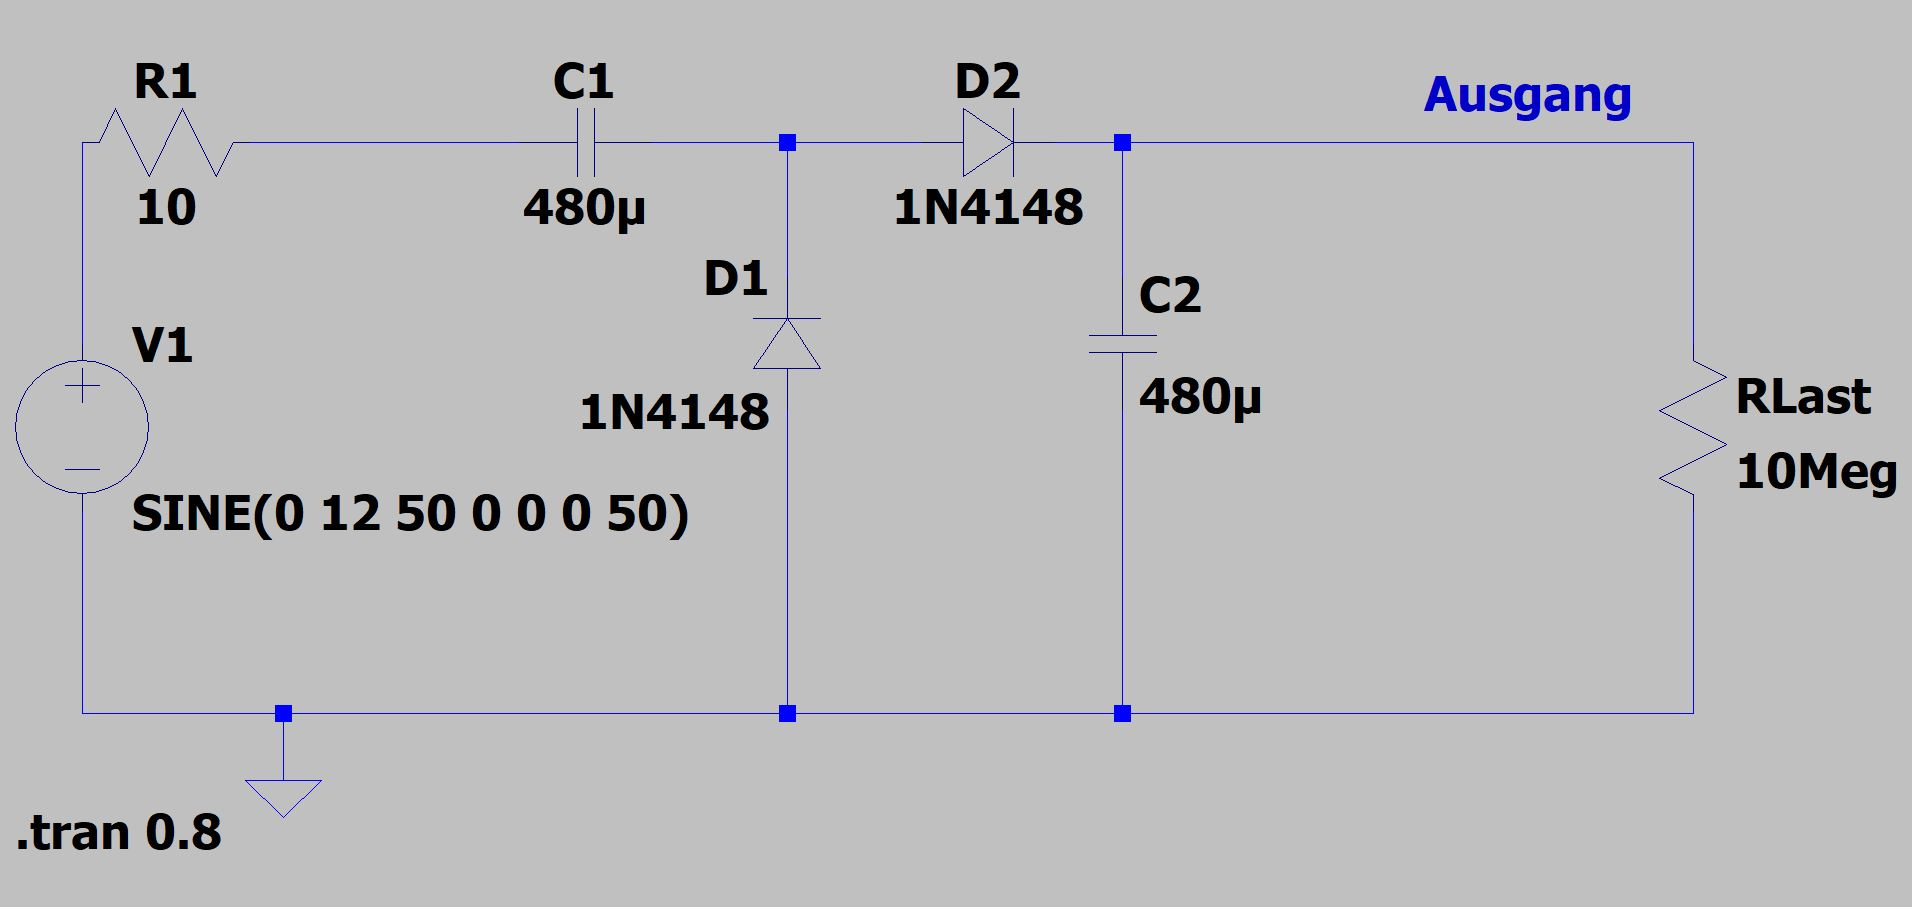
\includegraphics[width=\textwidth]{data/bspschaltung}
	\caption{Spannungsverdoppler}
	\label{bspS}
\end{figure}

\newpage

Der Kondensator C1 wird während der ersten positiven Halbperiode auf die Eingangsspannung, also die Spannung $u_{e}$, aufgeladen. In der darauf folgenden negativen Halbperiode findet nun ein Ladungsaustausch zwischen der Kondensatoren C1 und C2 statt. Die Diode D1 schließt sich und die Diode D2 öffnet sich. Dadurch fließt ein Strom über C2 zurück zur Spannungsquelle. C1 wird hierbei entladen und lädt den Kondensator C2 auf. Die Spannung an C2 beträgt am Ende der Periode den Wert der Eingangsspannung $u_{e}$. \\
Bei der nächsten positiven Halbperiode wird der Kondensator C1 wieder auf die Eingangspannung geladen, beim Wechsel zur negativen Halbperiode wird C1 auf die halbe Spannung entladen, C2 jedoch auf den 1,5-fachen Wert. Dies führt sich so weiter fort, bis die Spannung an C2 den doppelten Wert der Eingangsspannung erreicht hat.
\\ \\
Der doppelte Wert der Eingangsspannung wird nicht erreicht, da der Spannungsabfall bei einer Silizium Diode ca. $0,7\:$\si{\volt} beträgt. In der gegeben Schaltung sind zwei Dioden verbaut, deshalb liegt der Spannungsabfall bei ca. $1,4\:$\si{\volt}. 
\\ \\ 
Vergrößert man bei der Schaltung den Ladewiderstand, so beobachtet man in der Abbildung \ref{grossEin}, dass die Spannung am Ausgang bzw. am Kondensator C2 langsamer steigt.Dies ist dadurch zu begründen, dass durch den erhöhten Ladewiderstand ein geringerer Stromfluss möglich ist und damit der Ladungsausgleich verlangsamt wird. Durch die Verkleinerung des Lastwiderstands R2 kommt es bei der negativen Halbperiode auch zu einem Spannungsabfall am Kondensator C2, siehe Abbildung \ref{kleinLast}. Die Auswirkungen eines kleinen Lastwiderstandes mit großem Ladewiderstand sind in Abbildung \ref{fig:groKlein} graphisch dargestellt.

\begin{figure}
	\centering
	\begin{subfigure}[b]{\textwidth}
		\centering
		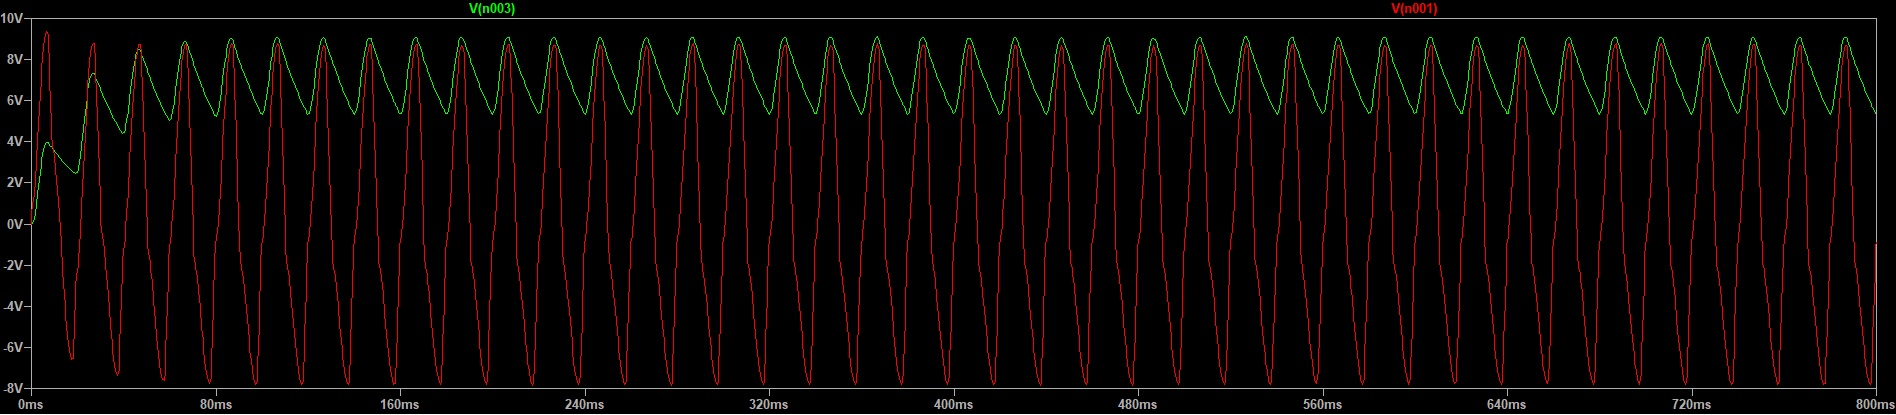
\includegraphics[width=\textwidth]{data/kleinLast}
		\caption{Spannungsverlauf bei kleinem Lastwiderstand}
		\label{kleinLast}
	\end{subfigure}
	\begin{subfigure}[b]{\textwidth}
		\centering
		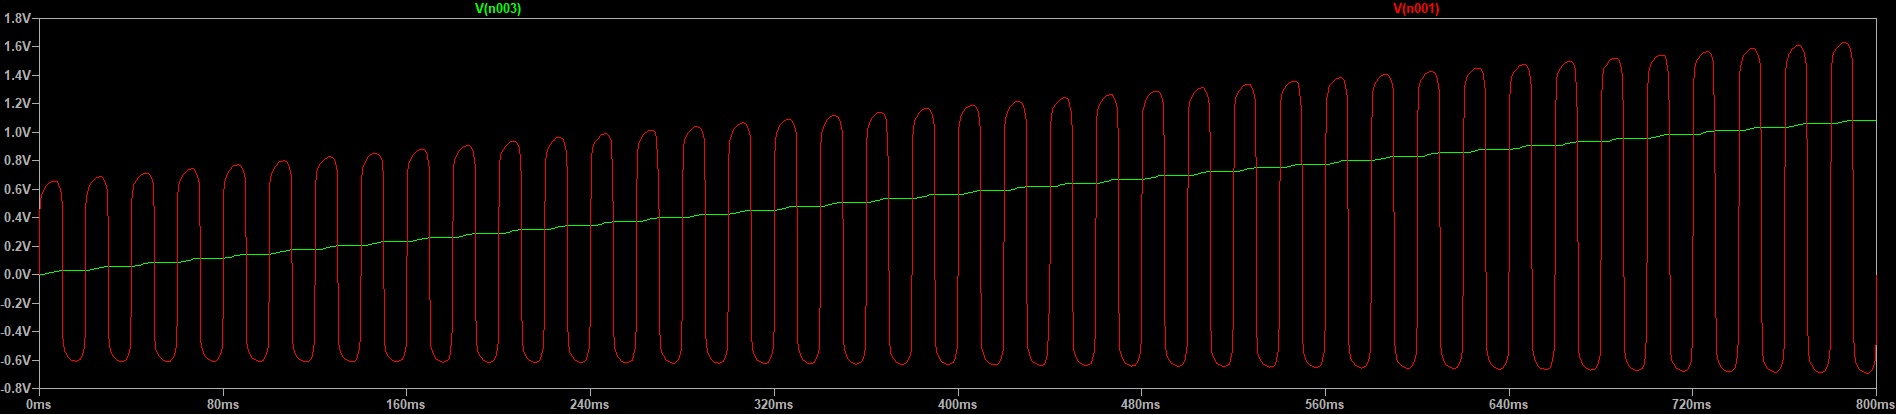
\includegraphics[width=\textwidth]{data/grossEin}
		\caption{Spannungsverlauf bei großem Ladewiderstand}
		\label{grossEin}
	\end{subfigure}
	\begin{subfigure}[b]{\textwidth}
		\centering
		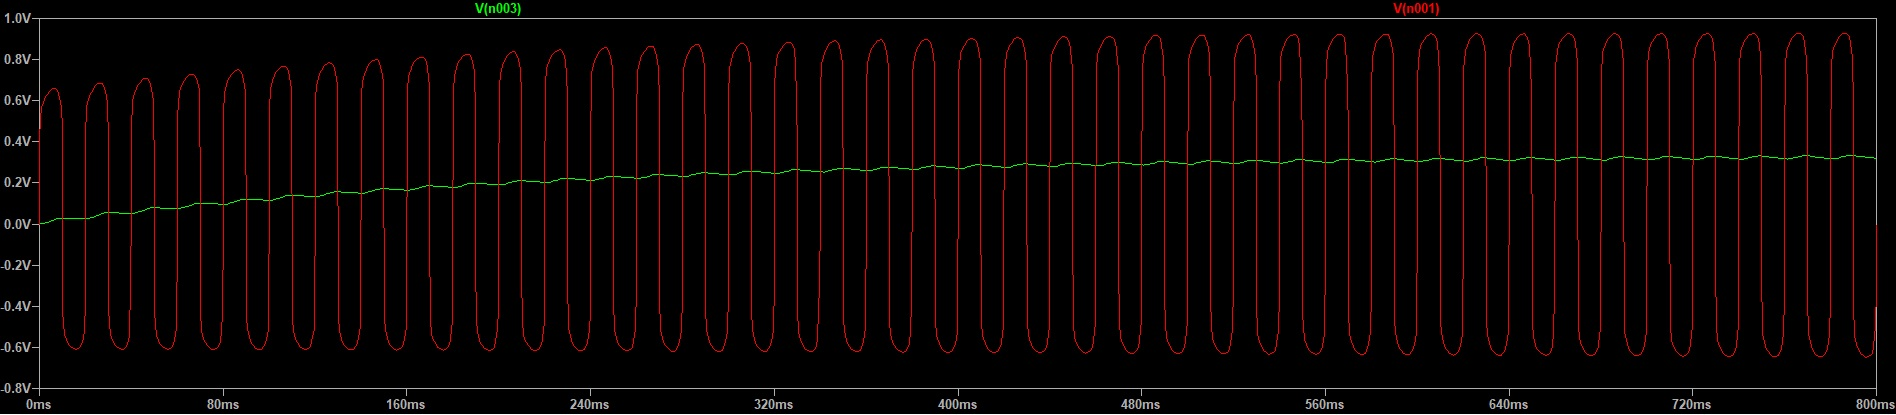
\includegraphics[width=\textwidth]{data/grossEin_kleinLast}
		\caption{Spannungsverlauf bei kleinem Lastwiderstand und großem Ladewiderstand}
		\label{fig:groKlein}
	\end{subfigure}
\caption{Verschiedene Spannungsverläufe, rot ist Spannung hinter dem Widerstand, grün die Ausgangsspannung}
\end{figure}
	\section*{Schaltungssimulation in Octave, Aufgabe 2.3}\label{sec:ag2.3}
Eine nummerische Simulation von linearen Schaltungen kann auch in Octave vor genommen werden. Hierzu wurden bereits die beiden Methoden \texttt{prs\_spice} (Methode zum Auslesen der Netzliste) und \texttt{dassl} (Methode zum nummerischen Lösen von Differenzialgleichungen) bereit gestellt.
Die Aufgabe wurde nun in 3 einzelne Skripte unterteilt:

\subsection*{Methode \texttt{circuit\_matrices}}
	Methode \texttt{circuit\_matrices} (siehe \ref{circuit_matrices}) berechnet alle Matrizen, die für die modifizierte Knotenanalyse benötigt werden. Rückgabewerte sind die Matrizen $\mathbf{A_C, A_L, A_R, A_V, A_I, C, L, G}$ sowie die Vektoren $\mathbf{v}$ und $\mathbf{i}$. Hierbei stellen die Variablen $\mathbf{A}$ so genannte Inzidenzmatrizen dar, also Matrizen, die Auskunft über die Beziehungen der Knoten und Kanten eines Graphen geben. In diesem Fall wird für jeden Typ Bauteil (Kondensator $C$, Spule $L$, Widerstand $R$, Spannungsquelle $V$ und Stromquelle $I$) eine Matrix erstellt, deren Einträge folgender Eigenschaft genügen:
	\begin{equation}
	a_{ij} = \begin{cases}
	+1 & \text{falls Zweig }j \text{ mit Bauteil von Knoten }i \text{ weg führt} \\
	-1 & \text{falls Zweig }j \text{ mit Bauteil zu Knoten }i \text{ hin führt} \\
	0  & \text{sonst}
	\end{cases}
	\end{equation}
	$\mathbf{C, L}$ und $\mathbf{G}$ stellen Diagonalmatrizen dar, die die Zahlenwerte der Bauteile enthalten (Induktivitäten in
	Henry, Kapazitäten in Farad, Leitfähigkeiten in Siemens). Zuletzt gibt die Methode die Vektoren $\mathbf{v}$ und $\mathbf{i}$ zurück, welche konstante Ströme oder Spannungen der Quellen enthalten.
	
\subsection*{Methode \texttt{calculate\_matrices}}
	Methode \texttt{calculate\_matrices} (siehe \ref{calculate_matrices}) setzt die zuvor berechneten Matrizen zu größeren Matrizen zusammen, die die Differenzialgleichung
	\begin{equation}
	\mathbf{M} \frac{\text{d}}{\text{d}t} \mathbf{x} + \mathbf{K} \mathbf{x} = \mathbf{r}
	\label{eq:matrixDGL}
	\end{equation}
	beschreiben. Rückgabewerte sind die Matrizen $\mathbf{M, K}$ und der Spaltenvektor $\mathbf{r}$, die sich nach folgender Rechenvorschrift ergeben:
	\begin{equation}
	\underbrace{
		\begin{bmatrix}
			\mathbf{A_C C A_C^T} & \mathbf{0} & \mathbf{0}\\
			\mathbf{0} & \mathbf{L} & \mathbf{0}\\
			\mathbf{0} & \mathbf{0} & \mathbf{0}
		\end{bmatrix}
	}_{\coloneqq \mathbf{M}}
	\frac{\text{d}}{\text{d}t}
	\begin{bmatrix}
		\boldsymbol{\varphi}\\
		\mathbf{i_L}\\
		\mathbf{i_L}
	\end{bmatrix}
	+
	\underbrace{
		\begin{bmatrix}
		\mathbf{A_R G A_R^T} & \mathbf{A_L} & \mathbf{A_V}\\
		-\mathbf{A_L^T} & \mathbf{L} & \mathbf{0}\\
		-\mathbf{A_V^T} & \mathbf{0} & \mathbf{0}
		\end{bmatrix}
	}_{\coloneqq \mathbf{K}}
	\begin{bmatrix}
	\boldsymbol{\varphi}\\
	\mathbf{i_L}\\
	\mathbf{i_L}
	\end{bmatrix}
	=
	\underbrace{
		\begin{bmatrix}
			-\mathbf{A_I i_S}\\
			\mathbf{0}\\
			-\mathbf{v_S}
		\end{bmatrix}
	}_{\coloneqq \mathbf{r}}
	\end{equation}
	\newpage

\subsection*{Finales Skript}	
	Das finale Skript (siehe \ref{finalesSkript}) löst nun die in \ref{eq:matrixDGL} beschriebene Differenzialgleichung auf nummerischen Weg. Dazu wird eine bereits in Octave implementierte Methode namens \texttt{dassl} verwendet. Diese bekommt den Term der Form $\mathbf{M} \frac{\text{d}}{\text{d}t} \mathbf{x} + \mathbf{K} \mathbf{x} - \mathbf{r}$ übergeben. Ebenso benötigt die Funktion die Anfangswerte $\mathbf{x_0}$ und $\mathbf{\dot{x}_0}$ sowie einen Vektor $\mathbf{t}$ mit Zeitpunkten, für die die Lösung berechnet werden sollen.

	Durch nummerische Annäherungsverfahren bestimmt die Methode den gesuchten Vektor $\mathbf{x}$ zum Zeitpunkt $t$. Dieser Lösungsvektor $\mathbf{x}$ enthält in diesem Fall die Werte
	\begin{equation}
	\mathbf{x} =
	\begin{bmatrix}
		\varphi_1\\
		\varphi_2\\
		i_L
	\end{bmatrix},
	\end{equation}
	also die beiden Potenziale $\varphi_1, \varphi_2$ an Knoten 1 und 2, sowie den Strom durch die Spule $i_L$ (siehe \ref{schaltplan}).
	Durch einzeichnen der verschiedenen Lösungen mithilfe der Methode \texttt{plot}, lässt sich der zeitliche Verlauf des Systems betrachten:
	
	\begin{figure}[h]
		\centering
		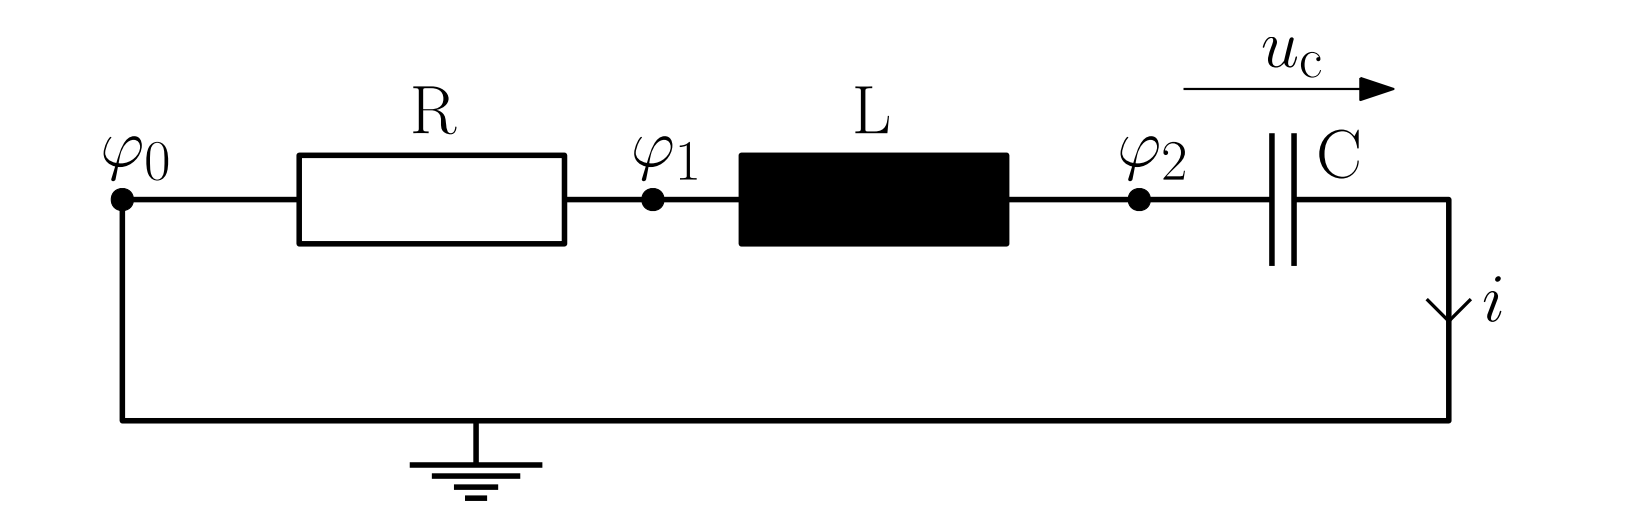
\includegraphics[width=0.65\textwidth]{data/schaltplan}
		\caption{\centering Schaltplan des harmonischen Oszillators mit $R=2\si{\ohm}$, $L=1.73007\si{\milli\henry}$ und $C=10\si{\micro\farad}$}
		\label{schaltplan}
	\end{figure}
	
	\begin{figure}[t]
		\centering
		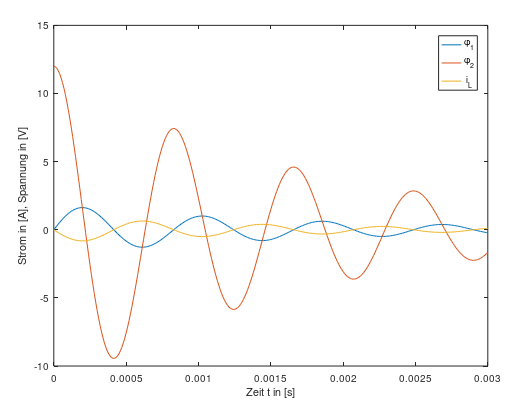
\includegraphics[width=0.76\textwidth]{data/plot}
		\caption{Schaltungssimulation des harmonischen Oszillators in \ref{schaltplan}. Initialisiert mit Anfangsspannung $u_C = 12V$ am Kondensator zum Zeitpunkt $t = 0$ }
		\label{plot}
	\end{figure}
\newpage
Hierbei entspricht $\varphi_1 = -u_R$ (der negativen Spannung am Widerstand), $\varphi_2 = u_C$ (der Spannung am Kondensator) und $i_L = i$ (Identisch zum Gesamtstrom, da es nur einen Strom im System gibt).

Hinweis zu den in \ref{finalesSkript} berechneten Anfangswerten $\mathbf{x_0}$ und $\mathbf{\dot{x}_0}$:

Diese müssten theoretisch per Hand für jede neue Schaltung und Art der Initialisierung des Systems neu berechnet werden. Jedoch scheinen auch inkorrekte Anfangswerte zum selben Ergebnis zu führen, was uns daraus schließen ließ, dass das numerische Annäherungsverfahren der \texttt{dassl}-Funktion, auch bei teilweise falschen Anfangswerten, zum richtigen Ergebnis konvergieren kann.

	%%%%%%%%%%%%%%%%%%%%%%%%%%%%%%%%%%%%%%%%%%%%
	
	%%%%%%%%%%%%%%%%%%%%%%%%%%%%%%%%%%%%%%%%%%%%%%%%%%%%%%%%%%%%%%%%%%%%%%%%%%%%%%%%%%%%%%%%%%%%%%%%%%
	
	%%%%%%%%%%%%%%%%%%%
	%Abbildungs- und Tabellenverzeichnis
	%%%%%%%%%%%%%%%%%%%
	\listoffigures % Abbildungsverzeichnis (captions in den Figuren werden als Referenz genommen)
	\listoftables % Verzeichnis der Tabellen (captions in den Tabellen werden als Referenz genommen)
	
	%%%%%%%%%%%%%%%%%%%
	%Literaturverzeichnis an dieser Stelle
	%%%%%%%%%%%%%%%%%%%
	
	
\end{document}
